The constant $c_s$ model was chosen as the model to test PTtools with,
as the model is the next logical extension of the bag model,
and there is some reference data available from \cites{giese_2020}{giese_2021}.
Figure \ref{fig:fluid_profiles} demonstrates solutions for three different wall speeds $v_\text{wall}$ and two different $\alpha_n$.
% These are not the same as the values \cite[fig. 10]{hindmarsh_gw_pt_2019}.
Instead of using only the bag model $c_{s,s}^2 = c_{s,b}^2 = \frac{1}{3}$,
each plot has four curves, each corresponding to a different combination of the sound speeds
$c_{s,s}^2 \in \{ \frac{1}{3}, \frac{1}{4} \}, c_{s,b}^2 \in \{ \frac{1}{3}, \frac{1}{4} \}$.
The corresponding gravitational wave spectra are plotted in \ref{fig:gw_spectra}.
Converting these to the frequencies today results in the figure \ref{fig:omgw0},
which also contains the LISA instrument noise spectrum as a reference.

\begin{figure}[ht!]
\centering
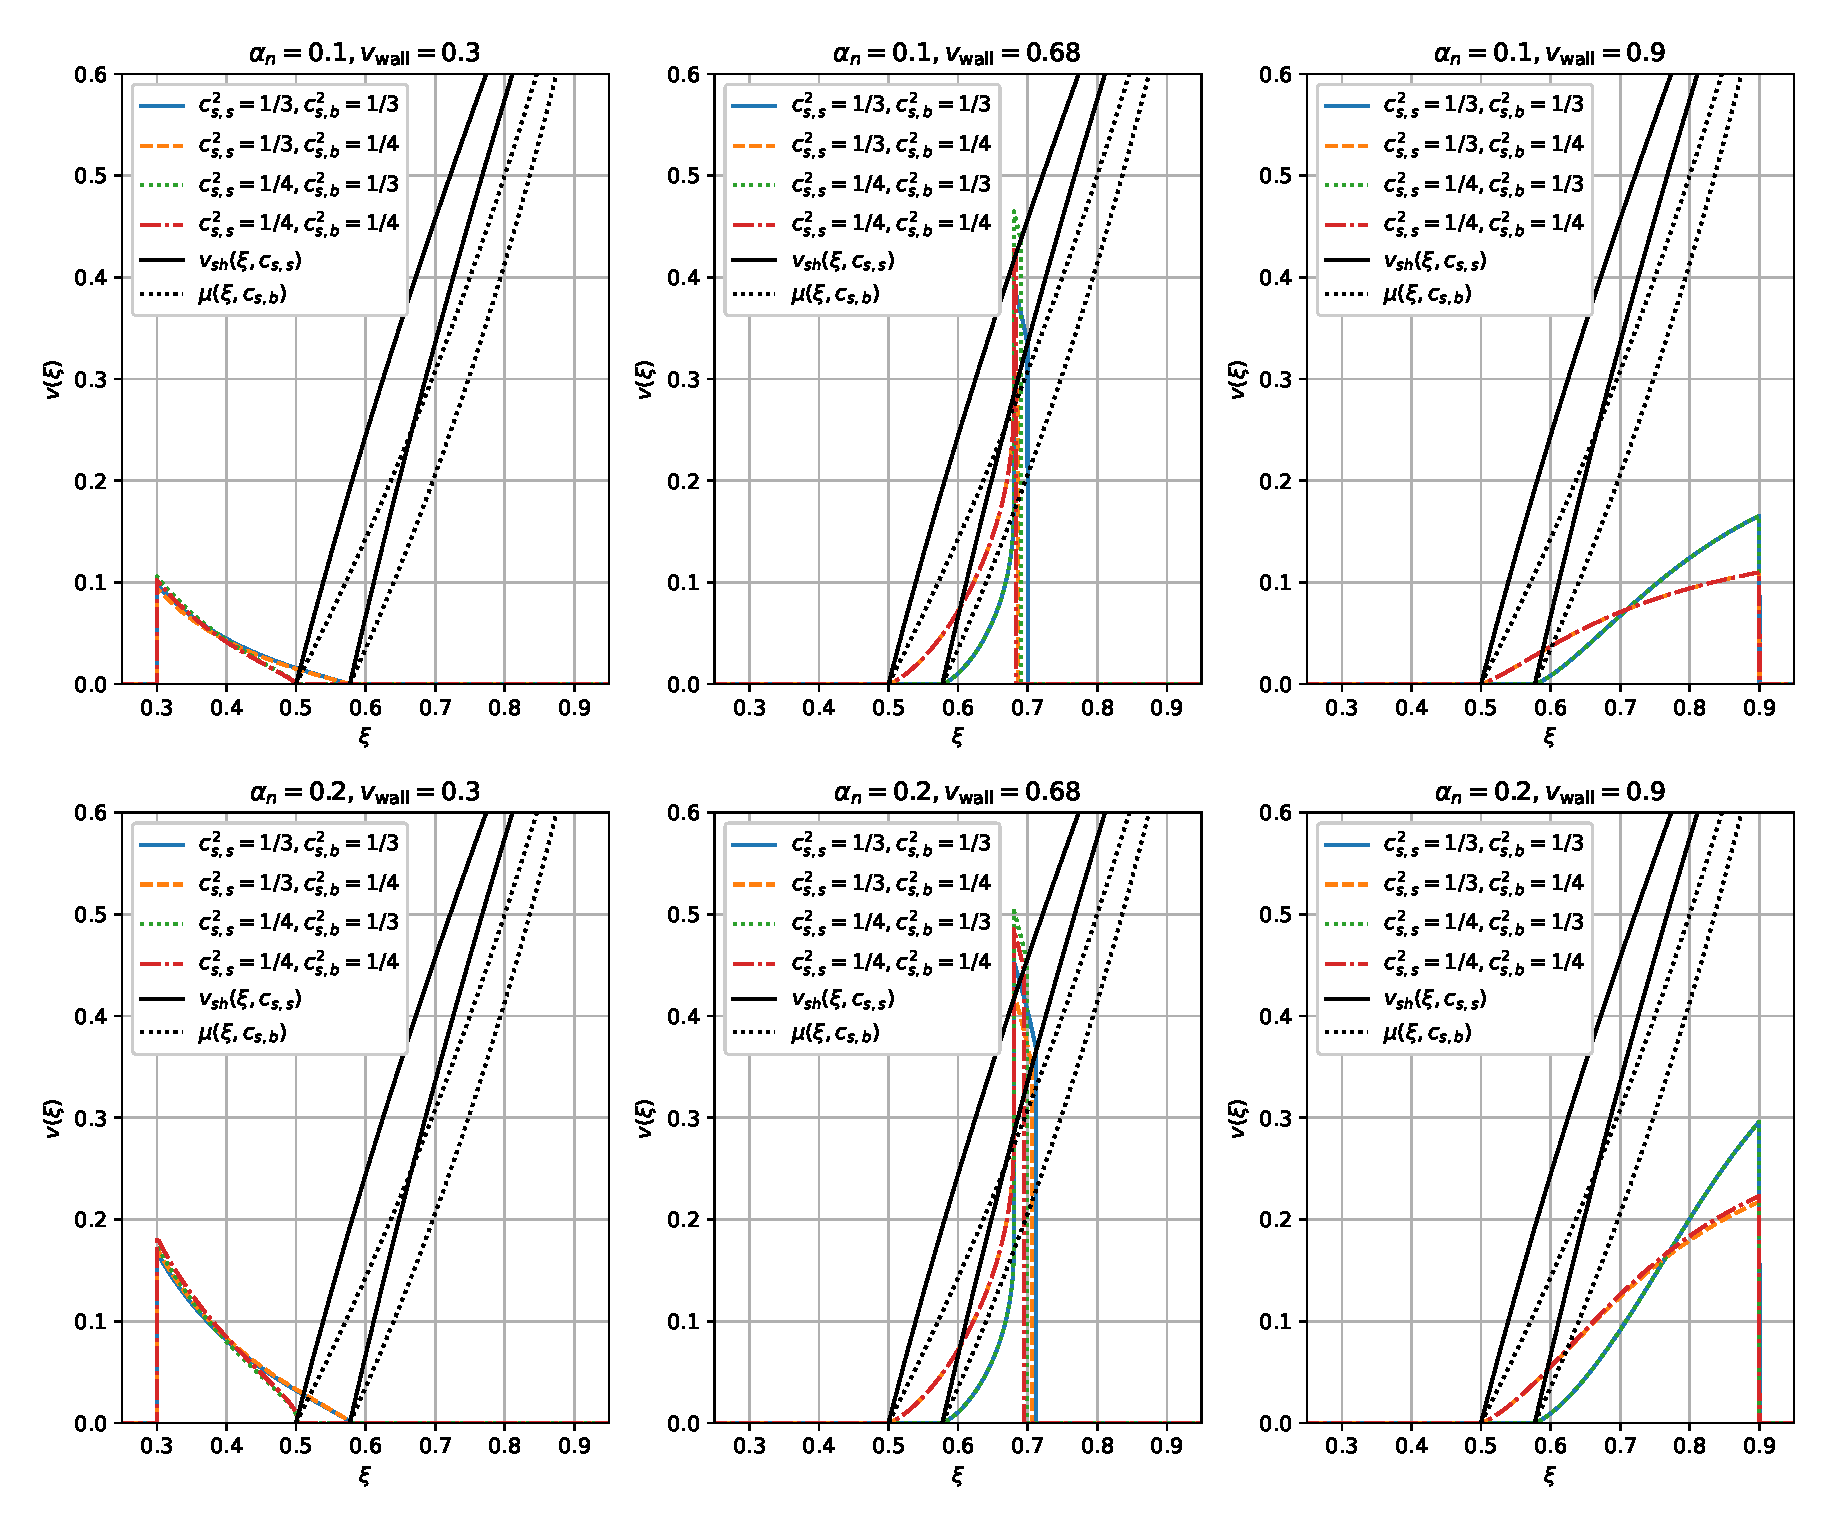
\includegraphics[width=\textwidth]{../pttools/examples/fig/const_cs_gw_v.eps}
\caption{Self-similar fluid profiles}
\label{fig:fluid_profiles}
\end{figure}

\begin{figure}[ht!]
\centering
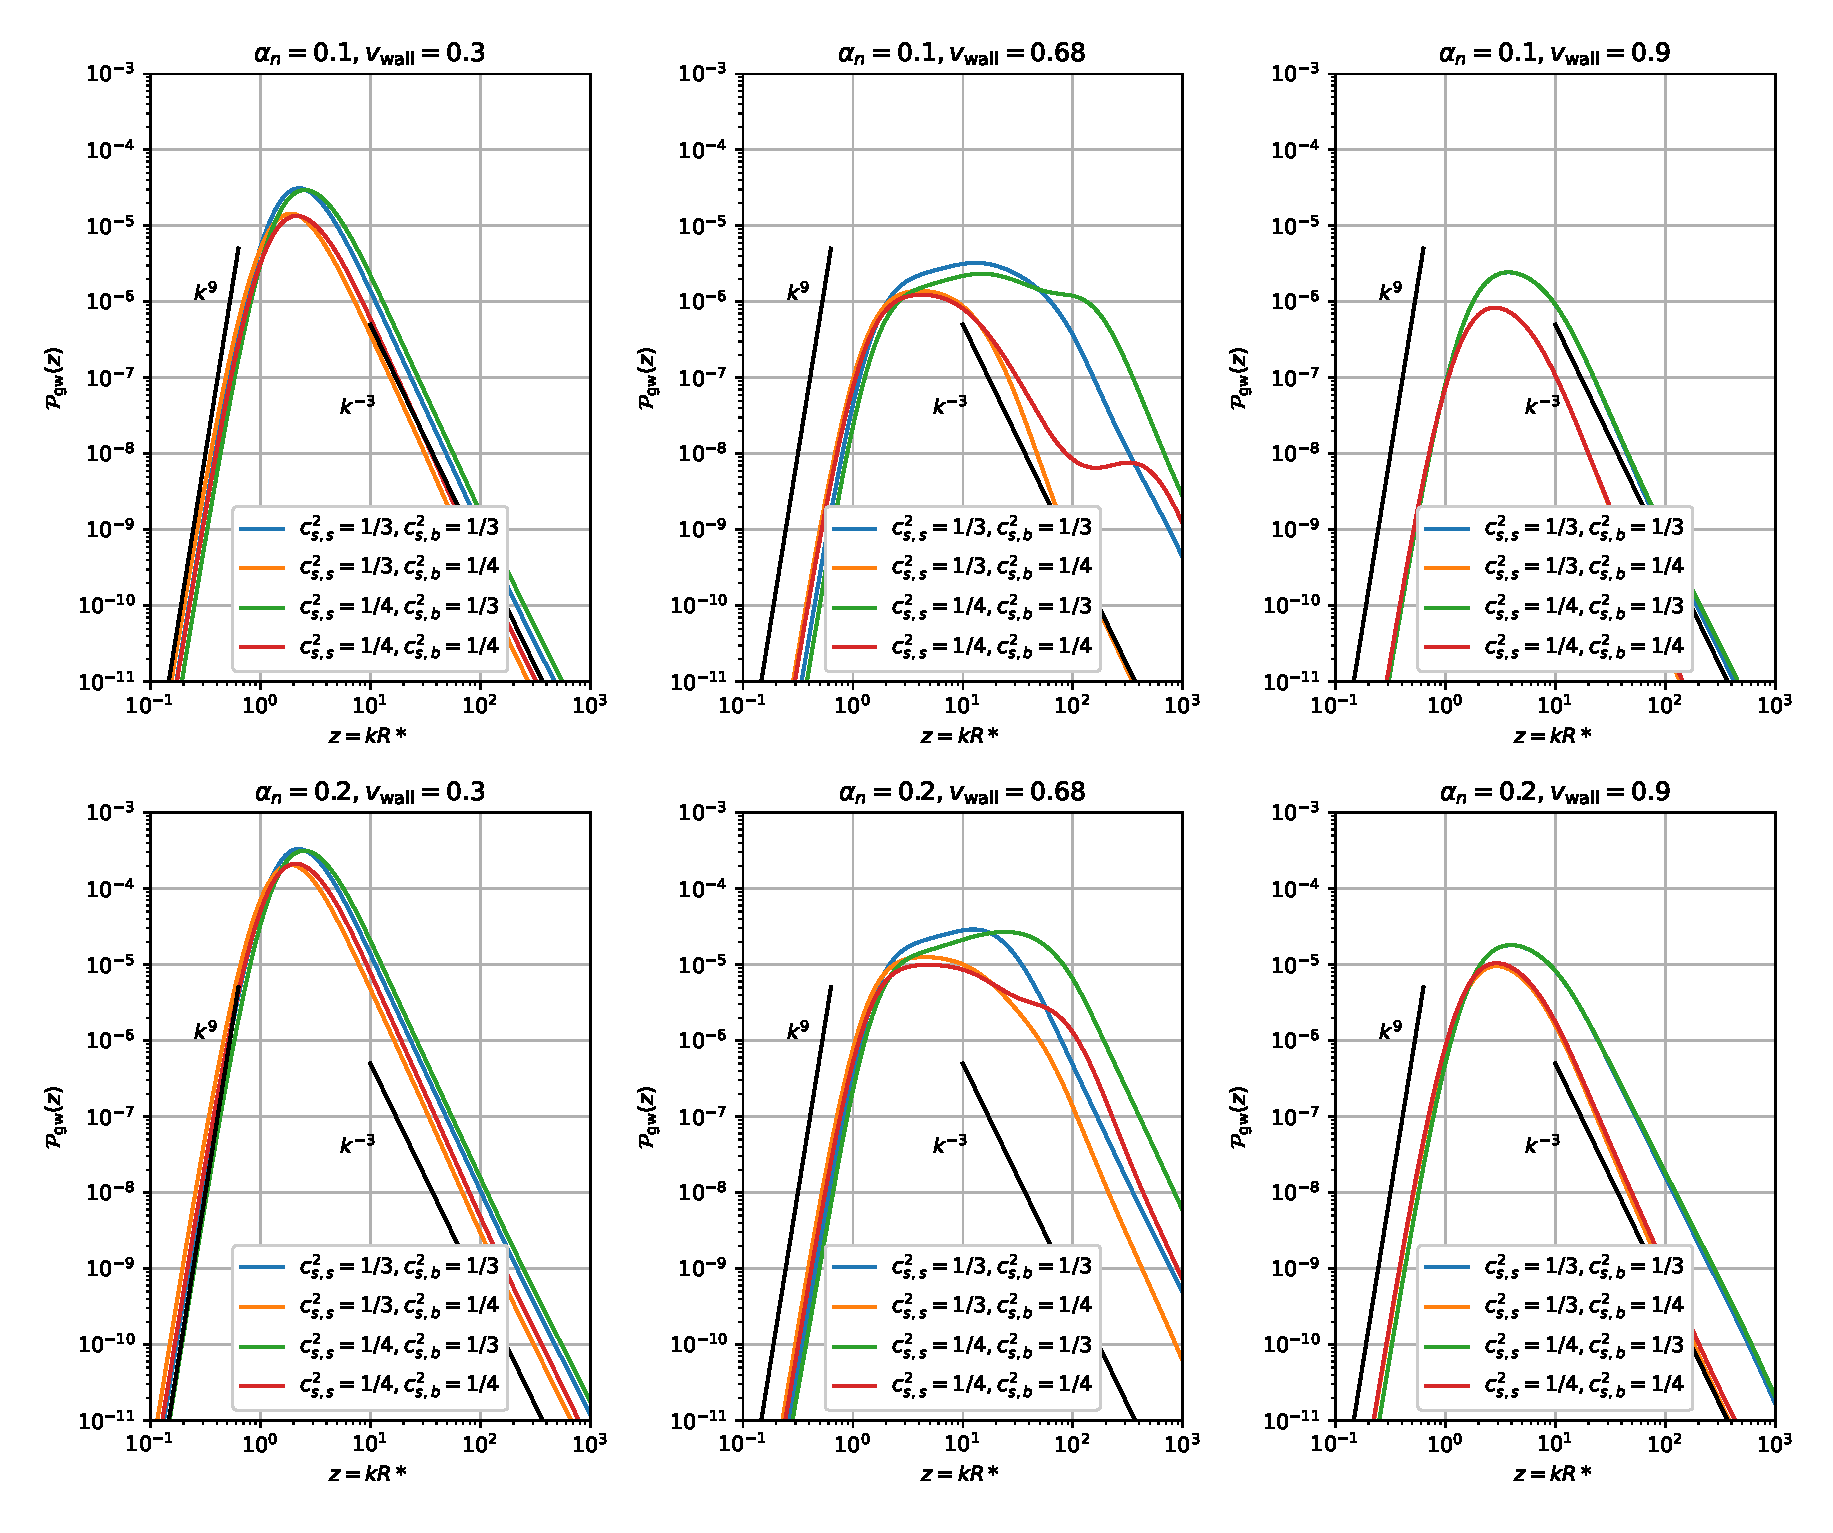
\includegraphics[width=\textwidth]{../pttools/examples/fig/const_cs_gw.eps}
\caption{Gravitational wave power spectra}
\label{fig:gw_spectra}
\end{figure}

\begin{figure}[ht!]
\centering
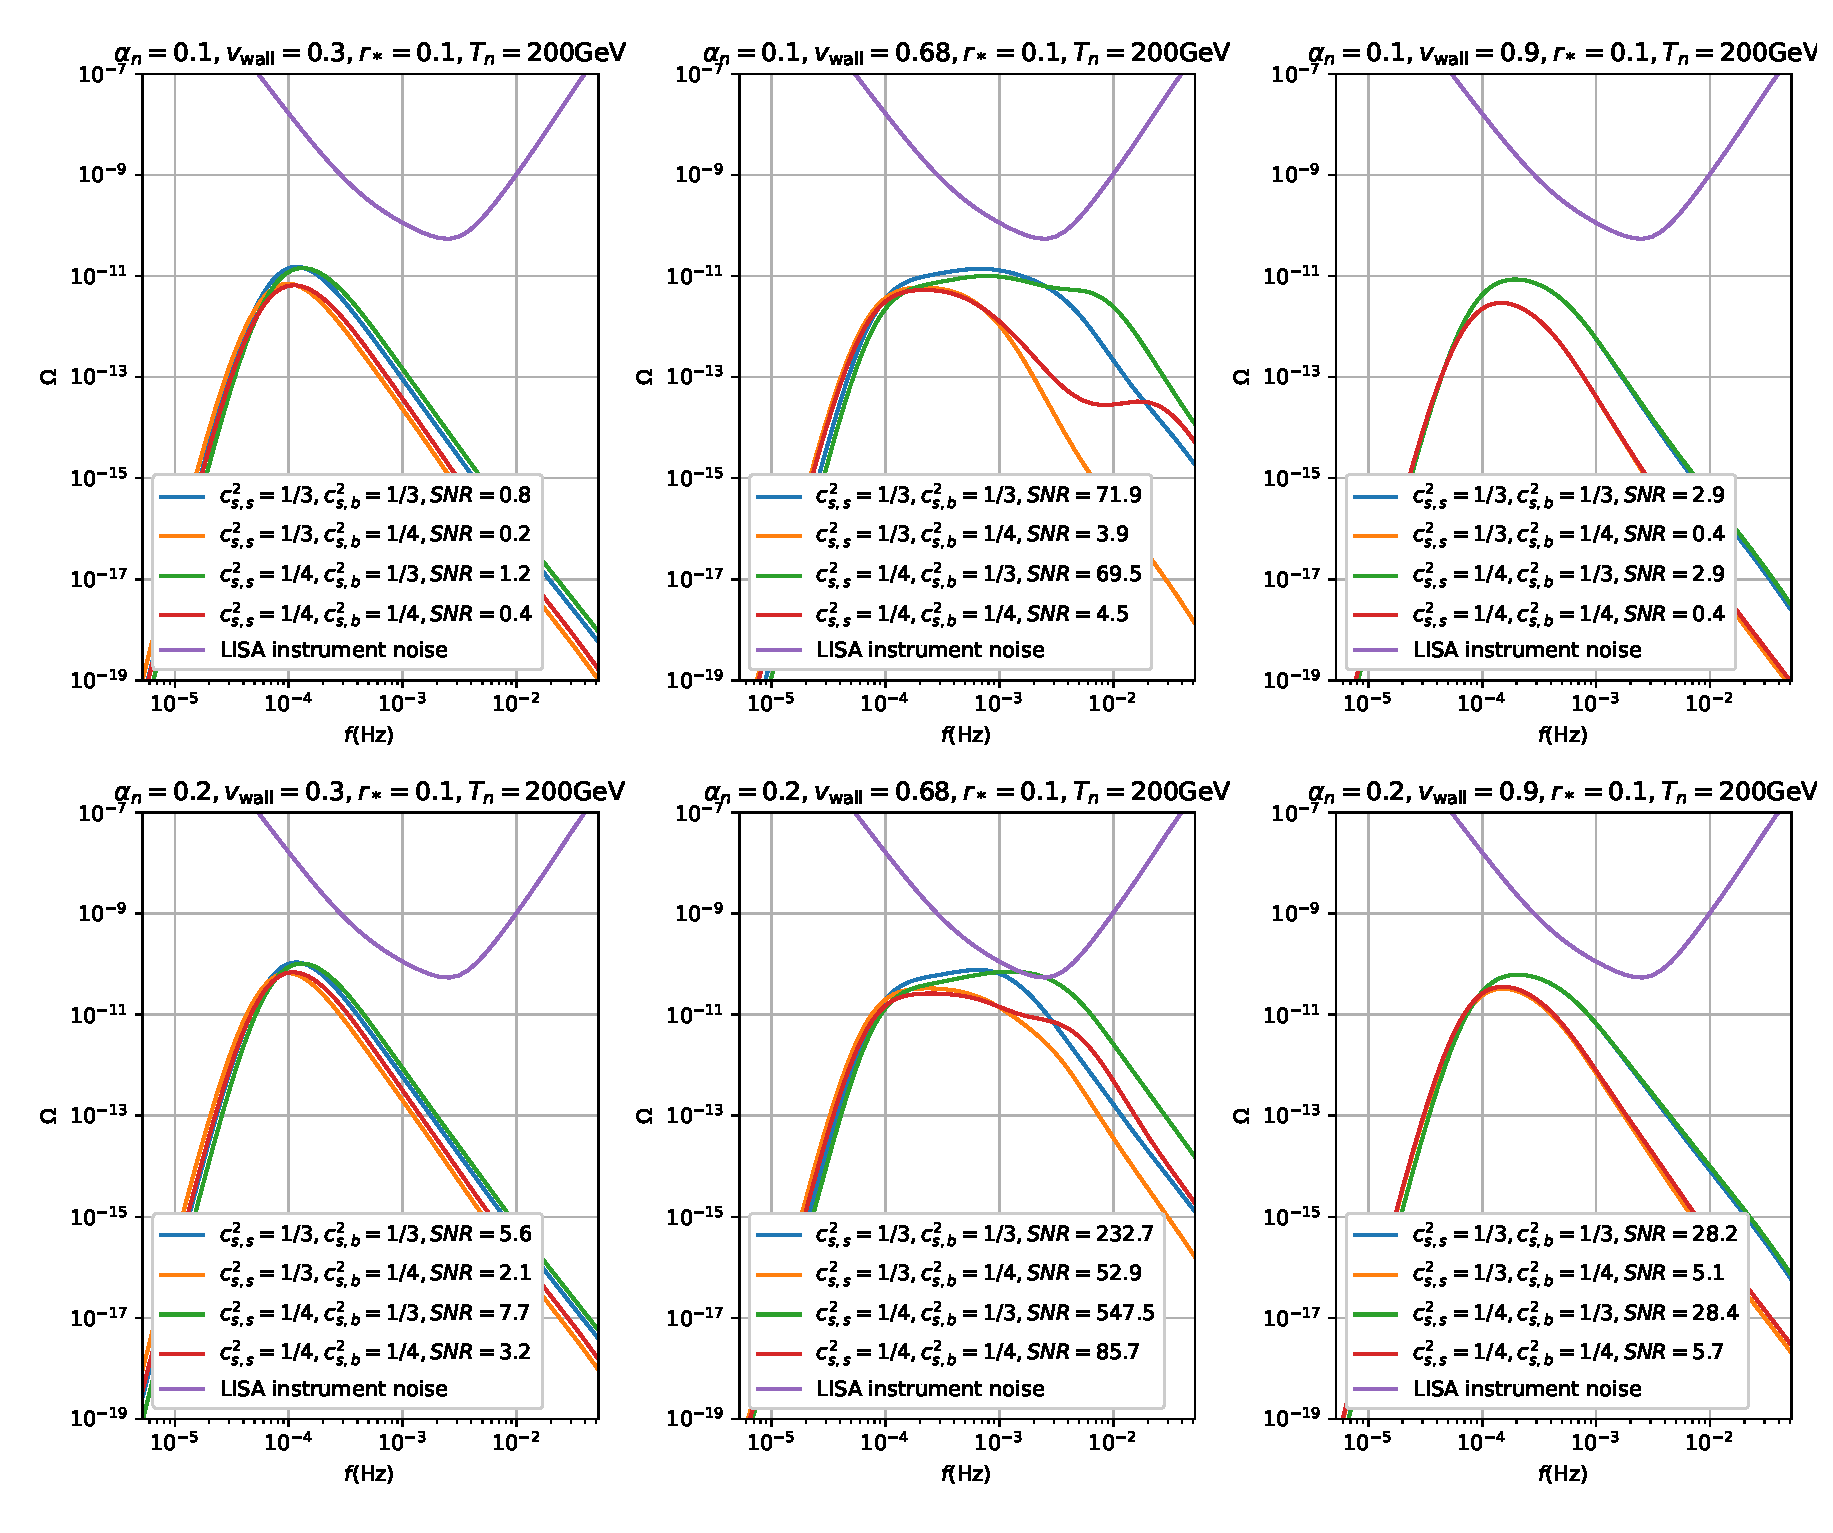
\includegraphics[width=\textwidth]{../pttools/examples/fig/const_cs_gw_omgw0.eps}
\caption{Gravitational wave power spectra today $\Omega_{gw,0}$}
\label{fig:omgw0}
\end{figure}

These figures demonstrate that the sound speed can have a profound effect on the resulting gravitational wave spectrum.
To understand how the sound speeds affect the gravitational wave spectrum,
we have to first study the fluid shells of figure \ref{fig:fluid_profiles}.

There are two curves that constrain the shape of the fluid shells.
The solid black curves are the shock velocities $v_{sh}(c_{s,s})$ that are determined by $c{s,s}$.
In general the shock velocity isalso dependent on $w$, since in general $c_s = c_s(w,\phi)$,
but in the constant sound speed model the sound speed is independent of the enthalpy.
Therefore we can plot the shock velocities as curves in the 2D plots instead of having to plot them as surfaces as functions of $(\xi,w)$ in a 3D plot.
The dotted black curves are the $\mu(\xi,c_{s,b})$ curves of eq. \eqref{eq:mu} that constrain the maximum fluid velocity inside the bubble.
They are dependent on the choice of $c_{s,b}$.
The $v_{sh}$ curves encounter $v=0$ at $\xi = c_{s,s}$ and the $\mu$ curves at $\xi = c_{s,b}$.

For all solution types, adjusting either of the sound speeds affects the degrees of freedom and therefore the pressure $p$ and enthalpy $w$ for that phase.
This affects the solution of the bubble wall junction conditions of eq. \eqref{eq:junction_condition_1}, \eqref{eq:junction_condition_2} and therefore $v(\xi_\text{wall})$,
which is also the peak of the fluid velocity profile.
This effect can be seen at the top-left figure, where all four fluid shells have different $v(\xi_\text{wall})$.
The change caused by adjusting the sound speed is the most profound for deflagrations when $c_{s,s}$ is decreased below $v_\text{wall}$, as it causes them to become hybrids, and vice versa.
Similarly changing $c_{s,b}$ so that the Chapman-Jouguet speed of \eqref{eq:chapman_jouguet} is decreased below $v_\text{wall}$ converts a hybrid to a detonation, and vice versa.
This can be seen at the top-right figure.

For deflagrations and hybrids, adjusting $c_{s,s}$ affects the location of the shock and therefore the thickness of the fluid shell.
It also affects the shape of the ODE integration and therefore the shape of the fluid shell in front of the bubble wall.
These effects can be seen at the top-left and bottom-left figures, where the curves with the same $c_{s,s}$ are grouped together.
Correspondingly for hybrids, adjusting $c_{s,b}$ affects $\mu(\xi_\text{wall},c_{s,b})$,
which is the point from which the integration of the detonation-like part of the fluid shell starts.
This can be seen in the two figures at the middle, where the detonation-like tails of the curves with the same $c_{s,b}$ are grouped together.
And for both detonations and hybrids, adjusting $c_{s,b}$ affects the shape of the fluid shell behind the wall.

These differences in the shapes of the fluid shells carry over to the gravitational wave spectra of fig. \ref{fig:gw_spectra} and eventually of the gravitational wave spectra today in fig. \ref{fig:omgw0}.
The sine transformation that converts ASDFASDF

To test the precision and reliability of the results provided by PTtools,
we compared to the results in \cite[fig. 2]{giese_2021},
resulting in figure \ref{fig:kappa_giese}.
It should be noted that the article uses $\kappa_{\bar{\theta}_n}$ of eq. \eqref{eq:kappa_thetabar_n},
which differs from the $\kappa$ defined in eq. \eqref{eq:kappa_omega}.
The colors from blue to gray correspond to $\alpha = 0.01, 0.03, 0.1, 0.3, 1, 3$.
The figures on the left have $\alpha = \alpha_{\bar{\theta}_n}$
and the figures on the right have $\alpha = \alpha_n$.
For each color, the upper line has $c_{s,b}^2 = \frac{1}{3}$ and the lower line $c_{s,b}^2 = \frac{1}{4}$.
The solid lines correspond to $c_{s,s}^2 = \frac{1}{3}$ and the dashed lines correspond to $c_{s,s}^2 = \frac{1}{4}$.

\begin{figure}[ht!]
\centering
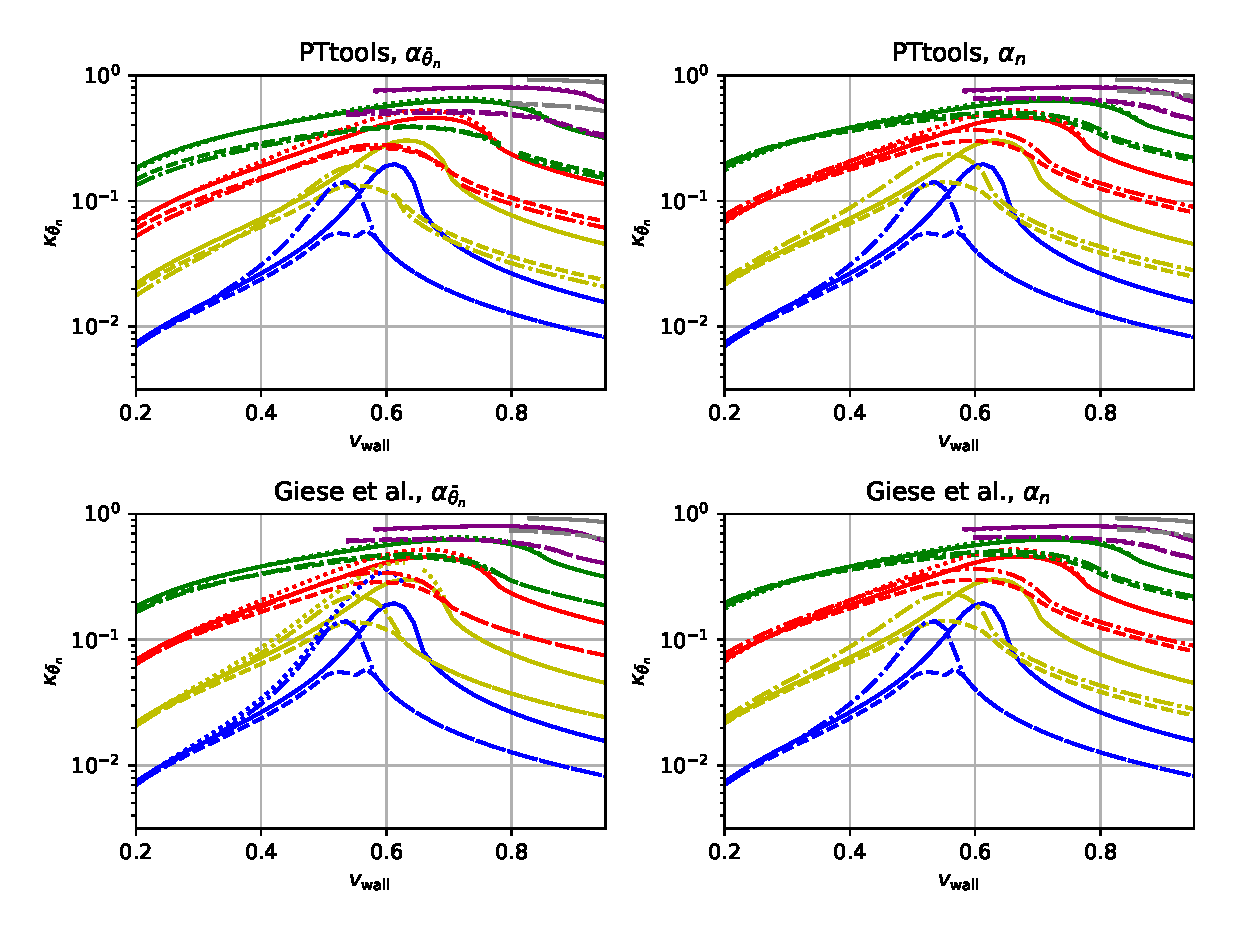
\includegraphics[width=\textwidth]{../pttools/examples/fig/giese_lisa_fig2.eps}
\caption{Comparison of $\kappa_{\bar{\theta}_n}$ values by \cite[fig. 2]{giese_2021} and PTtools}
\label{fig:kappa_giese}
\end{figure}
\todo{Use EPS instead of PNG}

It can be seen that PTtools and the code of \cite{giese_2021} produce results that are qualitativley similar, but slightly different.
This can be seen especially at the high wall speeds with $\alpha_n$ where changing $c_{s,s}$ (switching between the solid and dashed lines) has the opposite effect.

The gaps in the PTtools curves are caused by difficulties in finding a solution for very thin hybrid shells at the hybrid-detonation boundary.
It can happen that the shell is so thin that
It is also possible that the validity checks don't capture all the issues at this boundary,
resulting in a slightly wrong result.
This is demonstrated by the solid green $\alpha_n = 0.3, c_{s,s}^2 = \frac{1}{4}, c_{s,b} = \frac{1}{4}$ curve in the top-right figure.
These issues continue to be under investigation.

Some of the curves are not plotted by PTtools at all, since it has stricter tests for the validity of the bubble than the reference code.
One of such restrictions is that the $\alpha_n$ must be above the theoretical minimum for the model,
and that the model must have a valid critical temperature.
